\chapter{Passive Filters}

\section{Introduction}

In this lab, you will build and measure the performance of a low-pass
and a high-pass $RC$ filter, and produce Bode plots to compare your
circuit with the impedance model derived in class and shown in
Fig.~\ref{fig:bode}.  You will also build and measure the performance
of an $RLC$ band-pass filter and determine its resonant frequency and
quality (Q) factor. For this lab there are both logbook and Jupyter
notebook entries.

\begin{figure}[htbp]
\begin{center}
%\begin{tabular}{c@{\hskip 0.25in}c}
\begin{tabular}{cc}
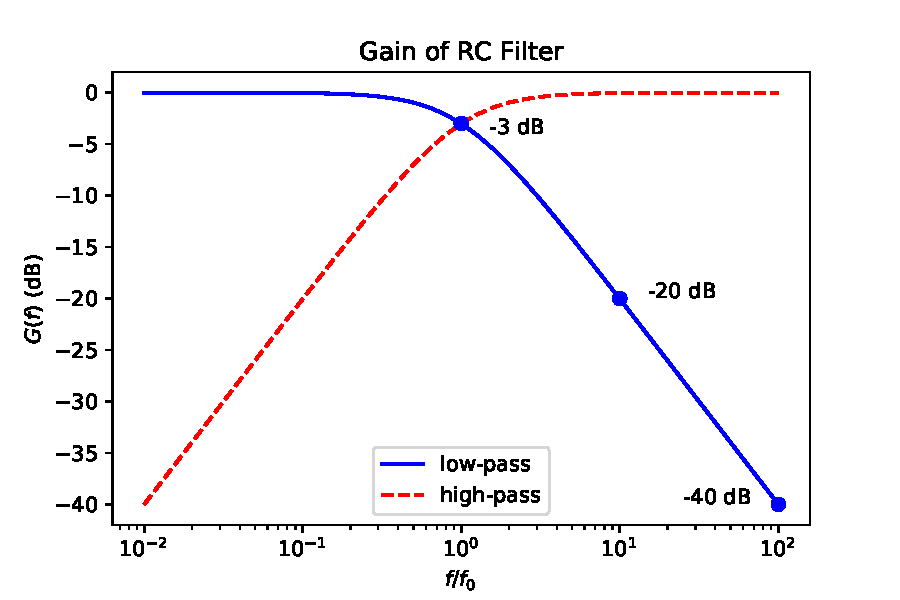
\includegraphics[height=0.22\textheight]{figs/labs/filters/rcgaindb.pdf}
&
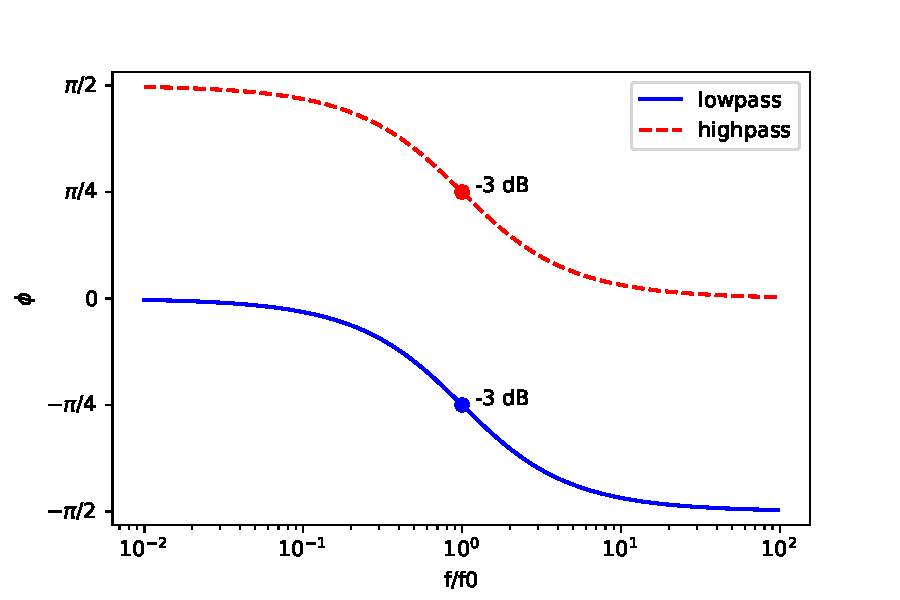
\includegraphics[height=0.22\textheight]{figs/labs/filters/rcphase.pdf} \\
(a) & (b) \\
\end{tabular}
\end{center}
\caption{\label{fig:bode} Bode plots for high-pass and low-pass filters showing the (a) gain on a dB scale, and (b) phase, both as a function of the ratio of frequency $f$ to the crossover frequency $f_0$ on a log scale.}
\end{figure}


\begin{figure}[htbp]
\begin{center}
\begin{tabular}{c@{\hskip 2cm}c}
\begin{circuitikz}[line width=1pt]
\draw (0,0) to[sinusoidal voltage source,bipoles/length=1.5cm] ++(0,4.0) to[short] ++(2.0,0) coordinate(X) to[short,*-o] ++(1.0,0) node[right]{C};
\draw (X) to[R,-*,l=$R_1$] ++(0,-2.0) coordinate(X) to[short,*-o] ++(1.0,0) node[right]{B};
\draw (X) to[C,-*,l=$C_1$] ++(0,-2.0) coordinate(X) to[short,-o] ++(1.0,0) node[right]{A};
\draw (X) to[short,-*] ++(-2.0,0) node[ground,yscale=2.0]{};
\end{circuitikz}  &
\begin{circuitikz}[line width=1pt]
\draw (0,0) to[sinusoidal voltage source,bipoles/length=1.5cm] ++(0,4.0) to[short] ++(2.0,0)coordinate(X) to[short,*-o] ++(1.0,0) node[right]{C};
\draw (X) to[C,-*,l=$C_1$] ++(0,-2.0) coordinate(X) to[short,*-o] ++(1.0,0) node[right]{B};
\draw (X) to[R,-*,l=$R_1$] ++(0,-2.0) coordinate(X) to[short,-o] ++(1.0,0) node[right]{A};
\draw (X) to[short,-*] ++(-2.0,0) node[ground,yscale=2.0]{};
\end{circuitikz}  \\
(a) & (b) \\
\end{tabular}
\caption{\label{fig:rc_circuits}
Circuit diagrams for $RC$ (a) low-pass filter and (b) high-pass filter.
The input voltage is $V_{\rm in} = V_{\rm AC}$ while the output voltage is $V_{\rm out} = V_{\rm AB}$.}
\end{center}
\end{figure}


\section{Low-pass Filters}

\begin{figure}[htbp]
\begin{center}
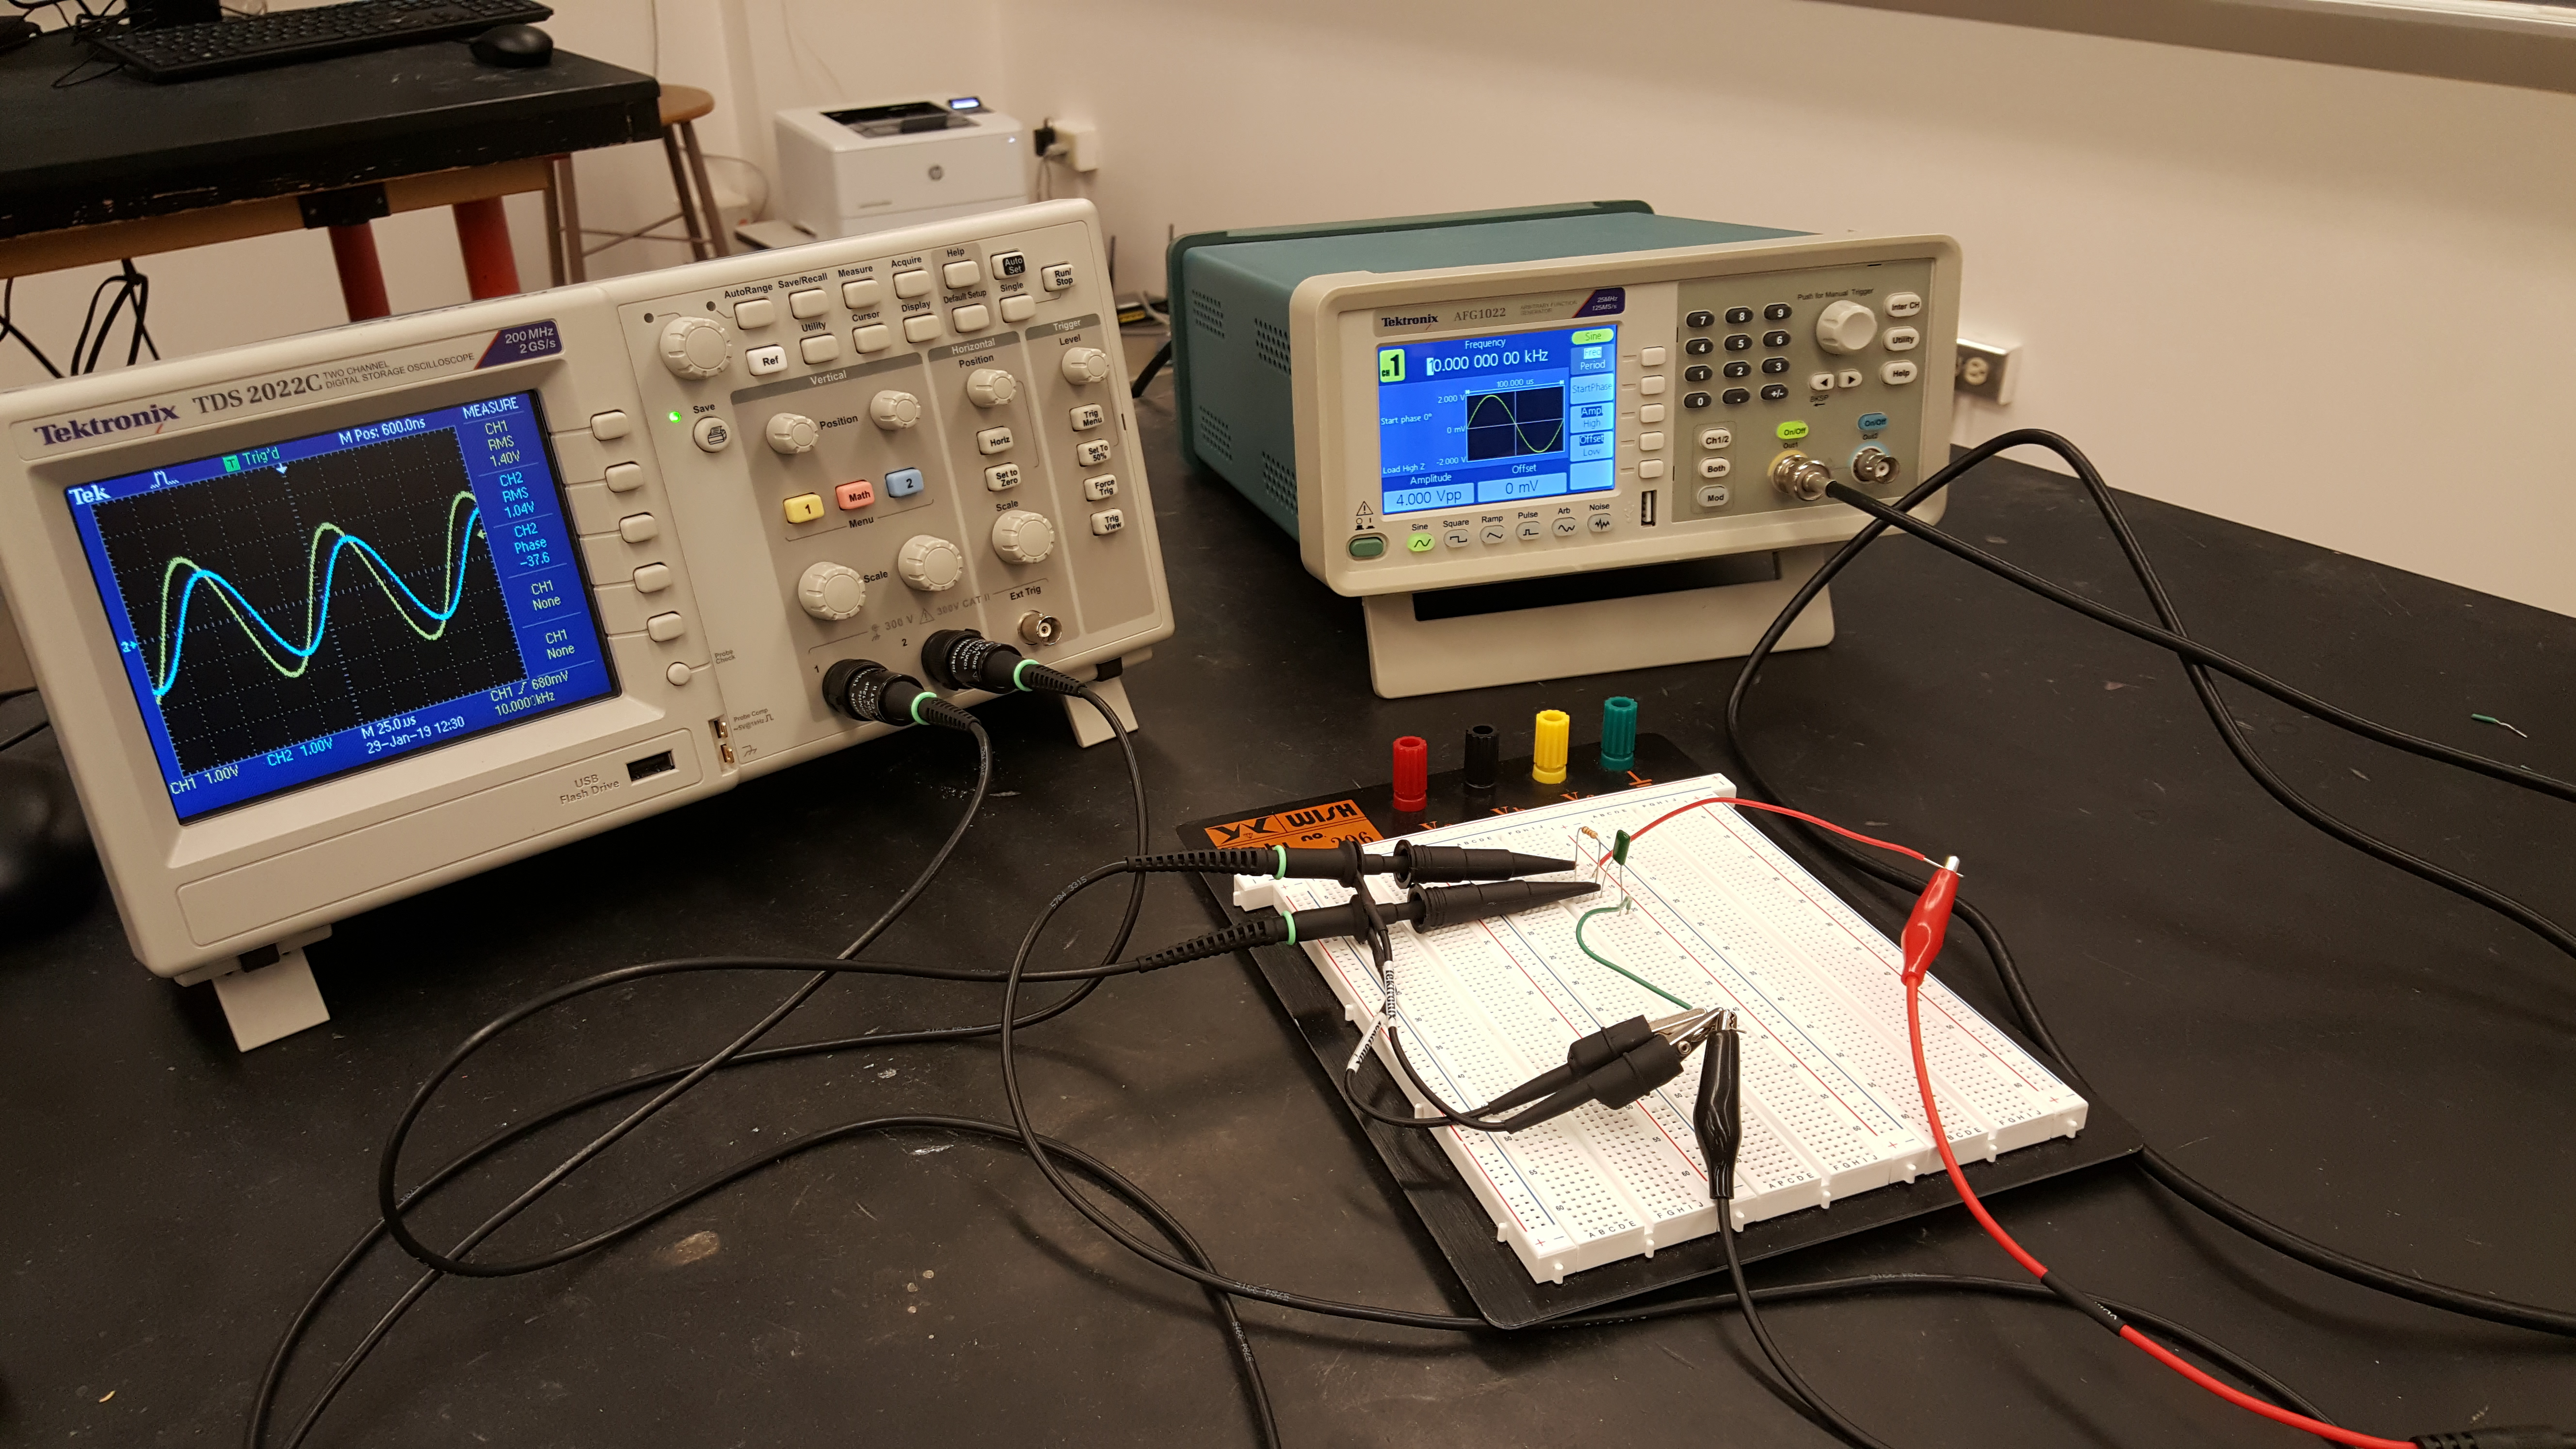
\includegraphics[height=0.22\textheight]{figs/labs/filters/filter_setup.jpg}
\end{center}
\caption{\label{fig:filter_setup} Setup for RC low-pass filter.}
\end{figure}


\begin{measurement} Calculate the corner frequency $f_0$ (aka the frequency of
$-3~\rm dB$ point) for the RC filters shown in
Fig.~\ref{fig:rc_circuits} for $R_1=1.5~\rm k\Omega$ and $C_1=10~\rm nF$.\\
\end{measurement}
\noindent Set your function generator to produce a sine function with a
peak-to-peak voltage of $4~\rm V$ and set the frequency to the calculated value of the corner frequency. %$10~\rmkHz$.  
Build the circuit shown in Fig.~\ref{fig:rc_circuits}a using
$R=1.5~\rm k \Omega$ and $C= 10~\rm nF$.  
\begin{measurement} Measure and record the
actual resistance and capacitance of the components before installing
them in your circuit. 
\end{measurement}
Use a BNC-alligator-pair cable to connect the
function generator output to your breadboard, to provide the AC
voltage source.  Keep in mind that the black alligator clip from your
function generator is earth ground, while the red alligator clip is the
function generator output referenced to ground, i.e. the top of the AC
source as drawn in the circuit diagram.

You will be using two scope probes in this lab, and as always some
care must be taken with respect to grounding when using your scope.
Your function generator has already set the earth ground point in your
circuit at the black alligator clip, which is point A in the circuit
diagram.  The scope grounding clips should both be connected to point
A.  To measure $V_{\rm in}$ on your scope Channel 1, connect the scope
probe tip of Channel 1 to point C in your circuit.  To measure $V_{\rm
  out}$ on your scope Channel 2, connect the scope probe tip of
Channel 2 to point B in your circuit.

The setup, including the scope, is illustrated in
Fig.~\ref{fig:filter_setup}.  Note in particular that the two scope
grounding clips and function generator ground are all connected to a
single (green) wire, which is used to set the ground point in the
circuit.

Set your Scope to the default setup, then adjust the timescale
appropriately and enable the output of channel 2.  
\begin{measurement} Calculate at $1\%$
precision the corner frequency $f_0$ from the measured values of your
resistor and capacitor, and set the frequency of your function
generator to that value. 
\end{measurement}

\noindent To produce the Bode plots for your filter,
we will be measuring the voltage gain $G = V_{\rm out} / V_{\rm in}$
and the phase shift $\phi$ of $V_{\rm out}(t)$ relative to $V_{\rm
  in}(t)$.

\begin{figure}[htbp]
\begin{center}
\begin{tabular}{cc}
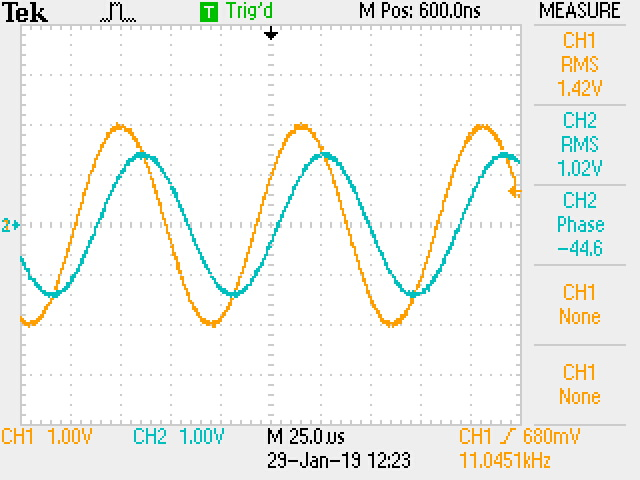
\includegraphics[width=0.4\textwidth]{figs/labs/filters/phase_measure.jpg} &
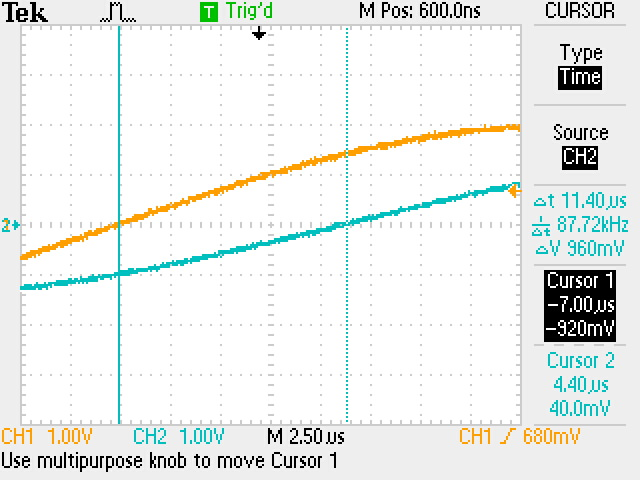
\includegraphics[width=0.4\textwidth]{figs/labs/filters/phase_cursor.jpg} \\
(a) & (b) \\
\end{tabular}
\end{center}
\caption{\label{fig:scopegain} Measuring the gain and phase with your scope.}
\end{figure}

The gain is the ratio of the amplitudes which can be read from the
scope traces.  Using the example in Fig~\ref{fig:scopegain}, the
output has an amplitude of 1.4 divisions while the input has an
amplitude of 2.0 divisions, so the gain is $G \sim 1.4/2.0 \sim
1/\sqrt{2}$.  After adjusting the horizontal scale and using the cursors menu, as
shown in Fig~\ref{fig:scopegain}, the offset in time $\Delta t$
between when each signals crosses zero is determined to be $11.4~\rm
\mu s$.  The offset in degrees is simply: 
\begin{displaymath}
\phi =  f_0 \, \Delta t \, \cdot (360^\circ).
\end{displaymath}
In this case, $\phi \sim 45^\circ$.  The phase can also be estimated
by noting that the output crosses zero half-way between where the
input crosses zero and its peak value, which is 1/8 of a period, or
$45^\circ$.  A gain of $1/\sqrt{2}$ and a phase-shift of magnitude
$45^\circ$ is expected at the cross-over frequency (or $-3~\rm dB$
point). Once you have estimated these quantities from the wave forms, you can
setup your scope to measure the appropriate quantities for you, using
the Measure menu, as shown in Fig.~\ref{fig:scopegain}.  The RMS
voltage measurement is generally the most reliable amplitude
measurement, so measure the RMS of each channel plus the phase
difference of channel 2 relative to channel 1.

\begin{measurement} 
Sketch the setup in your logbook. Measure and record the RMS amplitudes of channel 1 and channel 2, and the phase difference, at 
nine different frequencies, chosen to cover four orders of magnitude:
\begin{displaymath}
f=\{f_0/100, f_0/30, f_0/10, f_0/3,f_0, 3f_0, 10f_0, 30f_0, 100f_0\}
\end{displaymath}
where $f_0$ is the cross-over frequency.  You'll have to change the
horizontal scale appropriately as you change the frequency, as well as
the voltage scale for Channel 2 when the output is attenuated.  When
using the scopes automatic measurement functions, you should always
check at a few points by estimating the quantities yourself as shown
above.  You should note these cross-checks in your logbook. \end{measurement}

\section{High-pass Filter}

\begin{measurement} Sketch the setup in your logbook. Using the same components as in the previous section, build the
high-pass filter of Fig.~\ref{fig:rc_circuits}b, and repeat your
measurements at the nine different frequencies:
\begin{displaymath}
f=\{f_0/100, f_0/30, f_0/10, f_0/3,f_0, 3f_0, 10f_0, 30f_0, 100f_0\}
\end{displaymath}
\end{measurement}


\noindent
This is a \textbf{sign-off point} for this lab.

\section{Analysis}

\begin{plot} Plot the measured gain as a function of frequency for your high-pass
and low-pass filter, and compare to the expected response (using measured values of $R$ and $C$). 
Make sure to have
appropriate axis labels and a legend indicating ``Data'',``Prediction'',.... .
Use a more descriptive wording instead of Data and Prediction (given here only as example). 
Describe (in your Jupyter notebook) how those predictions are matching your measured data? \end{plot}

\begin{plot}  Plot the
measured phase shift as a function of frequency for your high-pass and
low-pass filter, and compare to the expected response. Make sure to have
appropriate axis labels and a legend indicating ``Data'',``Prediction'',.... .
Use a more descriptive wording instead of Data and Prediction (given here only as example). 
Describe (in your Jupyter notebook) how those predictions are matching your measured data?
\end{plot}

\begin{plot} Plot the measured gain \textbf{in decibels} as a function of frequency for your high-pass
and low-pass filter, and compare to the expected response (using measured values of $R$ and $C$). 
Make sure to have
appropriate axis labels and a legend indicating ``Data'',``Prediction'',.... .
Use a more descriptive wording instead of Data and Prediction (given here only as example). \end{plot}


\section{Band-pass Filter}

\begin{figure}[htbp]
\begin{center}
\begin{circuitikz}[line width=1pt]
\draw (0,0) to[sinusoidal voltage source,bipoles/length=1.5cm] ++(0,3.0) 
to[R,-*,l_=$R_1$] ++(2.0,0) coordinate(X) to[short,*-*] ++(1.5,0) coordinate(Y) to[short,-o] ++(1.0,0) node[right]{B};
\draw (X) to[C,-*,l=$C_1$] ++(0,-3.0)  to[short,-*] ++(-2.0,0) node[ground,yscale=2.0]{};
\draw (Y) to[L,-*,l=$L_1$] ++(0,-3.0)  coordinate(X) to[short,-*] ++(-1.5,0);
\draw (X) to[short,-o] ++(1.0,0) node[right]{A};
\end{circuitikz}  
\caption{Circuit diagram for RLC band-pass filter.}
\label{fig:rlc_circuit}
\end{center}
\end{figure}


%\begin{figure}[htbp]
%\begin{center}
%%\begin{tabular}{c@{\hskip 0.25in}c}
%\begin{tabular}{cc}
%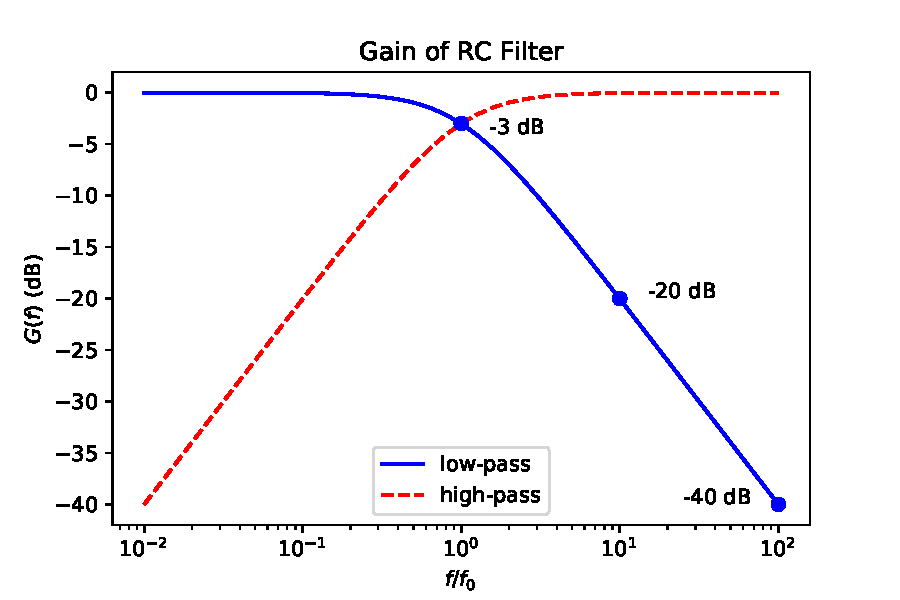
\includegraphics[height=0.22\textheight]{figs/labs/filters/rcgaindb.pdf}
%&
%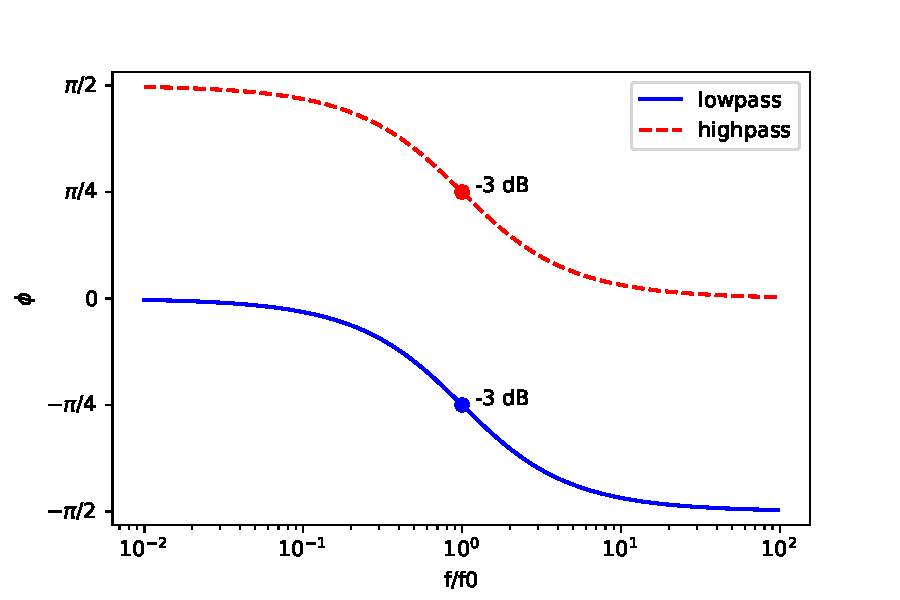
\includegraphics[height=0.22\textheight]{figs/labs/filters/rcphase.pdf} \\
%(a) & (b) \\
%\end{tabular}
%\end{center}
%\caption{\label{fig:bode} Bode plots for band-pass filter showing the (a) gain on a dB scale, and (b) phase, both as a function of the ratio of frequency $f$ to the crossover frequency $f_0$ on a log scale.}
%\end{figure}

%
%\begin{measurement} Calculate the resonant frequency:
%\begin{equation}
%f_0 = \frac{1}{2\pi \sqrt{LC}}. 
%\end{equation}
%of the resonant circuit in Fig.~\ref{fig:rlc_circuit}
%for $R_1=1.5~\rm k\Omega$, $C_1=10~\rm nF$, and $L_1 = 1~\rm mH$.
%\end{measurement}


%In lecture, we showed that the resonant angular frequency of an RLC
%band-pass filter is given by
%\begin{equation}
%\omega_0 = \frac{1}{\sqrt{LC}}. 
%\end{equation}
%At this frequency, the RLC resonant circuit has unit gain and no phase
%shift.  As the frequency moves away from the resonant frequency, the
%gain drops.  We define two points $\omega_+$ and $\omega_-$ as the two
%frequencies, one above and one below $\omega_0$, at which the gain
%drops below $1/\sqrt{2}$.  These are the two $-3~\rm dB$ points which
%define the bandwidth of the system.  We define the quality of the
%resonance by the ratio of resonant frequency to this bandwidth:
%
%\begin{displaymath}
%Q = \frac{\omega_0}{\omega_+ - \omega_-} = \frac{f_0}{f_+-f_-}
%\end{displaymath}

%For the RLC resonant circuit, we showed in lecture that:
%\begin{equation}
%Q = \omega_0 RC
%\end{equation}

\noindent Build the circuit in Fig.~\ref{fig:rlc_circuit} using $R=1.5~{\rm k \Omega}$ ,
$C=10~\rm{n F}$, and $L=1~\rm mH$. 
\begin{measurement} Using your DMM, measure and record
the actual resistance and capacitance of your components before
installing them. Use an LCR meter (BK Precision 878B)  to measure the actual inductance of the inductor and record it. Sketch the setup in your logbook.
Calculate $f_0$ using the measured values of your components. 
\begin{equation}
f_0 = \frac{1}{2\pi \sqrt{LC}}. 
\end{equation}
\end{measurement} 

\noindent Set the frequency of the function generator to $f_0$ and the peak-to-peak
voltage to $4~\rm V$.

\begin{figure}[htbp]
\begin{center}
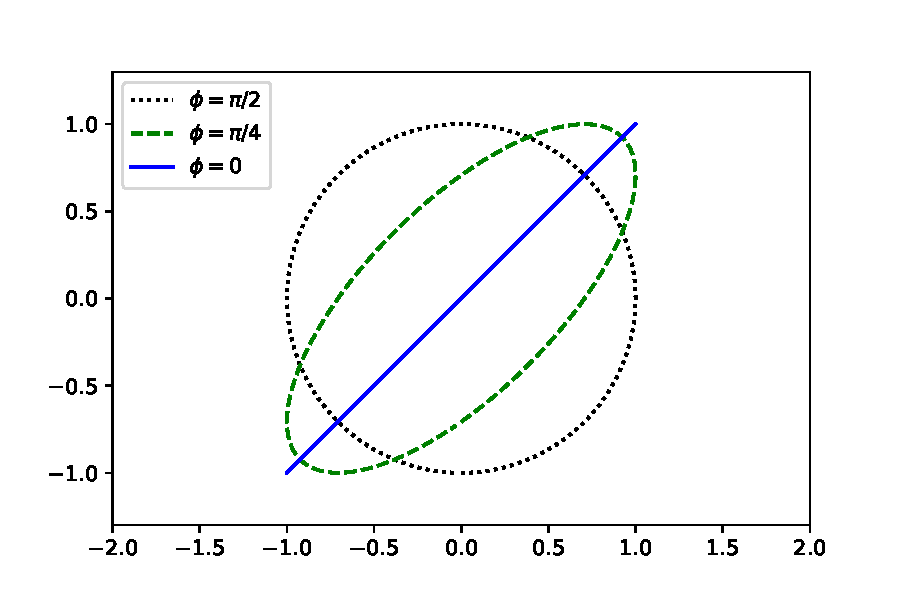
\includegraphics[width=0.50\textwidth]{figs/labs/filters/scope_xy.pdf}
\end{center}
\caption{\label{fig:scopexy} 
Expected scope traces in $XY$ display mode for a relative phase $\phi=\pi/2$, 
$\phi=\pi/4$, and $\phi=0$.  It is easy, accurate, and somehow deeply satisfying to tune the frequency until the ellipse collapses into itself, forming a line.}
\end{figure}

We'll measure the actual resonant frequency using a trick: an $XY$ mode of the scope.  
%During normal use, your oscilloscope displays the voltage of each channel versus
%time.  But there is an $XY$ mode available under the display options.
%In this mode, the scope displays the voltage of channel one versus the
%voltage of channel two.  
When in $XY$ mode, two out-of-phase signals
yield an ellipse.  But, as shown in Fig.~\ref{fig:scopexy} when both
channels are perfectly in phase, the ellipse collapses to make a
diagonal line. 
\begin{measurement} You can set you scope in XY mode and adjust the
frequency until the ellipse collapses to quickly and accurately find
the resonance frequency. Record the value in your logbook. Add comment in your logbook about how this measurement  compares to the calculated resonance frequency.
\end{measurement}
\begin{figure}[htbp]
\begin{center}
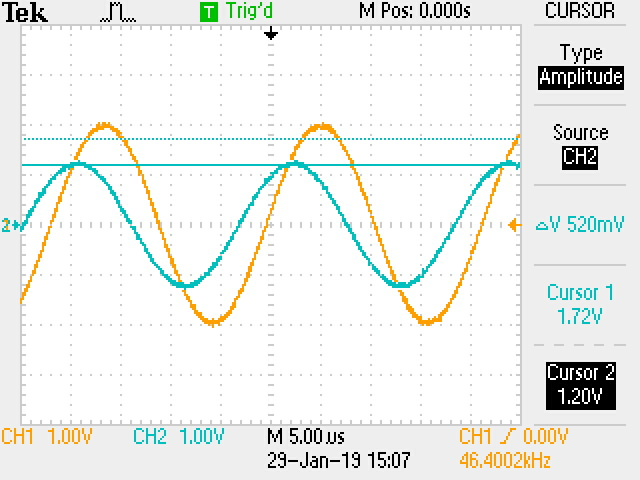
\includegraphics[width=0.45\textwidth]{figs/labs/filters/qscope.jpg}
\end{center}
\caption{\label{fig:qscope} Set Cursor 1 to the peak of Signal 2 at the resonant frequency, then set Cursor 2 to this value times $1/\sqrt{2}$.  The frequencies $f_+$ and $f_-$ can be determined by adjusting the frequency until the output amplitude reaches the level of Cursor 2, as shown here for $f_-$.
}
\end{figure}


\begin{measurement} One you determine the resonant frequency, switch back to the normal
display mode and determine the bandwidth.  The easiest way to obtain
this is to use the cursors to measure the peak voltage of your output
signal.  Multiply this by a factor of $1/\sqrt{2}$ to determine
the $-3~\rm dB$ amplitude and set the second cursor at this value, as
shown in Fig.~\ref{fig:qscope}.  Now adjust the frequency above and
below the resonant frequency and record at which frequencies the
amplitude reaches this line. Calculate the bandwidth and record it in your logbook.
\end{measurement}

\begin{measurement} From your measurement of $f_0$, $f_+$, and $f_-$ calculate the
measured $Q$-factor of your circuit. Record this value in your logbook. 
\end{measurement}


\noindent
This is a \textbf{sign-off point} for this lab. 
